\chapter{Interaction Region Local Coupling Correction in the LHC} % Main chapter title
\label{chapter:IR_Local_Coupling} % For referencing the chapter elsewhere, use \cref{chapter:IR_Local_Coupling}

Lot of stuff here should be from my PRAB article.
Some paragraph before the first section.

\begin{figure}
    \centering
    \includegraphics*[width=0.9\linewidth]{Figures/IR_Coupling_Correction/lhc_vs_hllhc_ratios_normalised.pdf}
    \caption{Relative increase in IP beam size from powering the left and right skew quadrupole correctors around the IP, for a \betastar of \qty{50}{\centi\metre} for the LHC and \qty{15}{\centi\meter} for the HL-LHC.}
    \label{figure:lhc_vs_hllhc_ratios}
\end{figure}

%----------------------------------------------------------------------------------------

\section{Local Betatron Coupling in the Interaction Regions}

\todo{In here I need a small subsection talking about the 2018 ion run issue.}

Mention that in the machine we have unavoidable tilt errors in the insertion region magnets.
A tilted quadrupole interacts with the beam as a straight quadrupole with an additional skew quadrupolar component.
This skew component will have an effect on the \foneohone resonance driving term given by~\cite{PRAB:Calaga:Coupling_Merging_Hamiltonian_Matrix_Approaches}:

\begin{equation}
    f(s)_{1001} = \frac{-1}{4 \left(1 - e^{2 \pi i \left(Q_x - Q_y \right)}\right)} \sum_l k L_l \sqrt{\beta_x^l \beta_y^l} e^{i \left(\Delta \phi_x^{s l} - \Delta \phi_y^{s l}\right)}
    \label{equation:skew_quad_contribution_to_f1001}
\end{equation}
where \(k L_l\) is the \(l^{\mathrm{th}}\) skew quadrupole integrated strength, \(\beta^l_{x,y}\) are the \betafunctions at the position of the \(l^{\mathrm{th}}\) quadrupole, \(\Delta \phi^{sl}_{x,y}\) are the phase advances between the measurement point and the \(l^{\mathrm{th}}\) quadrupole, and \(Q_{x,y}\) are the horizontal and vertical tunes.

As one can see in \cref{figure:ir5_and_around}, due to the very large \betafunctions in the triplet quadrupoles, tilts in these magnets have the potential to drastically contribute to the magnitude of the \foneohone term, and therefore to the coupling in the interaction region and, if not compensated properly, to the coupling in the whole machine.
In the LHC, a skew quadrupole corrector is installed on each side of colliding IPs, just before the third triplet quadrupole \(\mathrm{Q3}\) on the side of the IP.
Due to their location, these correctors are single aperture magnets meaning that both beams are passing through a single cavity, and feel the same magnetic field.
As the triplet quadrupoles - also single aperture magnets - are expected to be most of the contribution to local coupling, the local error to be corrected should be the same for both beams and such an arrangement of correctors is manageable.


Twiss with Coupling and Ripken parameters
Equivalency of Ripken and Tracking when looking at beam size

Below are plots / tables / equations to be included:

\begin{equation}
    \langle z \rangle = \sqrt{\varepsilon_{1} \beta_{1z} + \varepsilon_{2} \beta_{2z}}
    \label{equation:lebedev_beam_size}
\end{equation}
where \(z\) can be one of \(x\), \(y\), \(\varepsilon_{1}\) and \(\varepsilon_{2}\) are respectively the horizontal and vertical emittances.
The Ripken parameters are output directly from MAD-X.
The evolution of both the \AbsCminus and the beam size at IP for a given value of the quadrupole tilt error can be seen in \cref{fig:colin_correction_dqmin_lebedev}.

\begin{figure}
    \centering
    \includegraphics*[width=0.9\linewidth]{Figures/IR_Coupling_Correction/guess_rdts.pdf}
    \caption{Similarly looking coupling RDTs in the machine for two drastically different scenarii in terms of luminosity.}
    \label{figure:guess_rdts}
\end{figure}

\begin{figure}[!htb]
    \centering
    \includegraphics*[width=0.99\columnwidth]{Figures/IR_Coupling_Correction/round_lhcb1_ir1.pdf}
    \caption{LHC IR1 for a round optics configuration at 7~TeV and \(\beta^{*} = 25\)~cm. The upper plot shows the machine layout with dipoles in blue and quadrupoles in red. The lower plot shows \(\beta\) and dispersion functions for both transverse planes. The vertical green lines highlight the location of the skew quadrupole correctors used for corrections.}
    \label{fig:lhcb1_round_optics_ir1}
\end{figure}

\begin{table}[!hbt]
    \centering
    \begin{tblr}{colspec={ccccc}}
        \hline
        \textbf{Magnet} & \textbf{K\(_{1S}\) [m\(^{-2}\)]}    \\
        \hline
        MQSX.3R[IP] \(\rightarrow K_{1S}\)  &  \num{1E-4}   \\
        MQSX.3L[IP] \(\rightarrow K_{1S}\)  &  \num{-1E-4}  \\
        \hline
    \end{tblr}
    \caption{Definition of one unit of the colinearity knob, a powering setting of the IR skew quadrupole correctors.}
    \label{table:colin_knob}
\end{table}

\begin{figure}[!htb]
    \centering
    \includegraphics*[width=\columnwidth]{Figures/IR_Coupling_Correction/waist_shift_leaks_rdts.pdf}
    \caption{Linear coupling RDTs in the vicinity of IP1 under a coupling bump, with and without a rigid waist shift. The vertical green lines represent the positions of the skew quadrupoles (MQSX.3[RL]1) used to implement the coupling bump. A colinearity knob setting of 10 and a rigidity waist shift knob setting of 1 were used, which results in a \qty{0.5}{\percent} change in the triplet powering knob.}
    \label{fig:rdt_leak}
\end{figure}


\begin{figure}[!htb]
    \centering
    \includegraphics*[width=0.99\columnwidth]{Figures/IR_Coupling_Correction/colin_knob_vs_waist_shift.pdf}
    \caption{Impact of the colinearity knob on the global \AbsCminus with and without applying a rigid waist shift.}
    \label{fig:knob_to_cminus_with_waist}
\end{figure}


\begin{figure}[!htb]
    \centering
    \includegraphics*[width=0.99\columnwidth]{Figures/IR_Coupling_Correction/beam_size_colin_compensation.pdf}
    \caption{Resulting beam size increase for various combinations of tilt error and colinearity knob settings.}
    \label{fig:beam_size_comp}
\end{figure}

\begin{figure}[!htb]
    \centering
    \includegraphics*[width=0.99\columnwidth]{Figures/IR_Coupling_Correction/colin_correct_dqmin_lebedev_tilt4e-4.pdf}
    \caption{Resulting \AbsCminus and IP1 beam size, according to \cref{equation:lebedev_beam_size}, for various powering of the skew quadrupole correctors, after introducing a \qty{0.4}{\milli\radian} tilt error on the Q3s left and right of IP1. The black dotted line represents the threshold of a \qty{1}{\percent} beam size increase from the nominal scenario.}
    \label{fig:colin_correction_dqmin_lebedev}
\end{figure}

%----------------------------------------------------------------------------------------

\section{Current Correction Methods and Limitations}

Overview of IR Difficulties (phase advances suck, DFFT of x -jpx, no instruments, SbS errors)

%----------------------------------------------------------------------------------------

% \section{The Hunt for an Observable}

% \subsection{Combined RDTs}

% Some theory here (see Franchi's paper, see Michael's paper), it can use DFFT of x/y only.
% Some studies that it's difficult to use directly (2021.8), maybe SbS?

% \subsection{SbS with combined RDTs and that it works better than with RDTs?}

% \subsection{Forced RDTs}

% Why am I looking into this again?
% Potentially if I have time we can see if using non-compensated stuff gives better corrections.
% Very optional at the moment.

% \subsection{Conclusion that we might need to look at outside observables}

%----------------------------------------------------------------------------------------

\section{Rigid Waist Shift for Local Coupling Correction}

\subsection{Concept and Simulations}

% Whatever the choice is, remove the unused plots from the repo afterwards
\begin{figure}
    \centering
    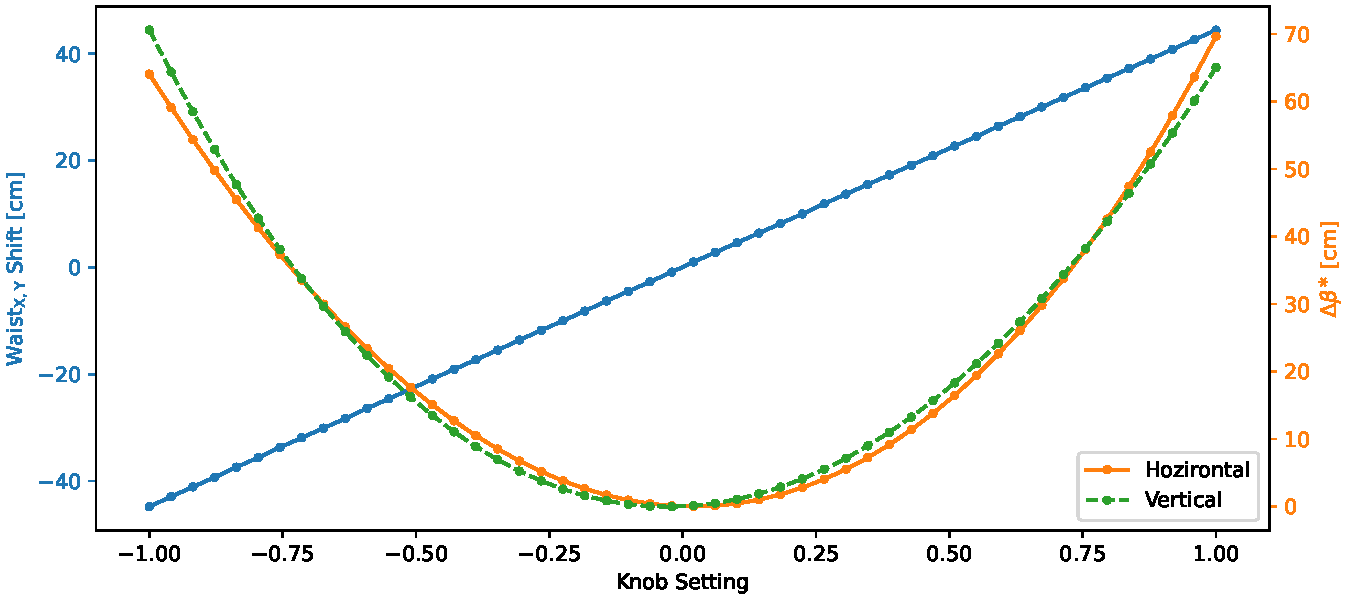
\includegraphics[width=0.9\textwidth]{Figures/IR_Coupling_Correction/rigid_waist_shift_effect_combined.pdf}
    \caption{Simulated effect of the designed rigid waist shift knob on the collision optics (\betastar of \qty{30}{\centi\metre}) in the horizontal and vertical plane. The blue line represents the waist displacement from the design location and is almost completely linear with the knob setting. The orange and green lines represent the horizontal and vertical \betafunctions change at the IP point itself as the waist is displaced, respectively. The minima of the parabolas are not found at the zero knob setting as the design optics include a very small waist.}
    \label{figure:rigid_waist_shift_knob_effect1}
\end{figure}

% Whatever the choice is, remove the unused plots from the repo afterwards
\begin{figure}[htp]
    \centering
    \subfloat[.9\linewidth][Horizontal plane]{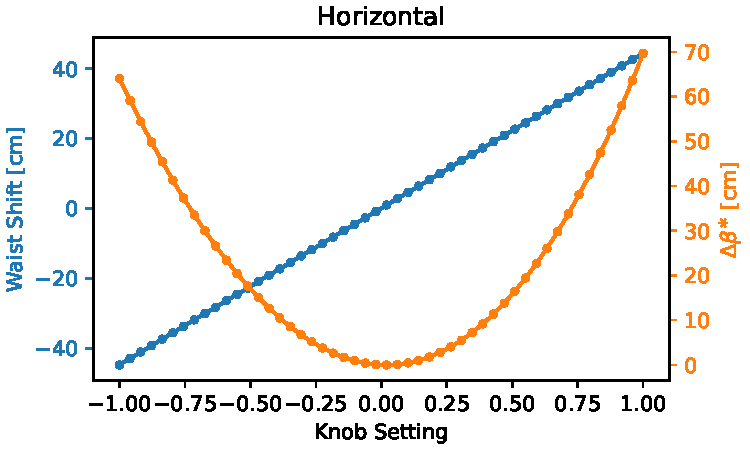
\includegraphics[width=7cm]{Figures/IR_Coupling_Correction/rigid_waist_shift_effect_horizontal.pdf}}
    \hspace{0.3cm}
    \subfloat[.9\linewidth][Vertical plane]{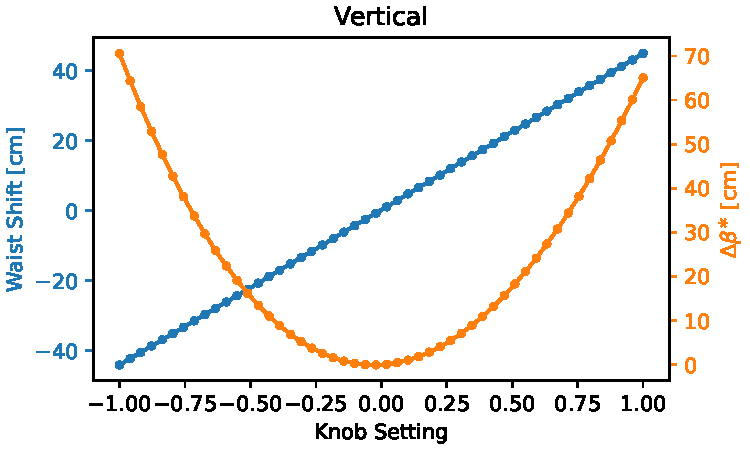
\includegraphics[width=7cm]{Figures/IR_Coupling_Correction/rigid_waist_shift_effect_vertical.pdf}}
    \caption{Simulated effect of the designed rigid waist shift knob on the collision optics (\betastar of \qty{30}{\centi\metre}) in the horizontal (left) and vertical (right) plane. The blue line represents the waist displacement from the design location and is almost completely linear with the knob setting. The orange line represents the \betafunction change at the IP point itself as the waist is displaced. The minimum of the parabola is not found at the zero knob setting as the design optics include a very small waist.}
    \label{figure:rigid_waist_shift_knob_effect2}
\end{figure}

\subsection{Determining Corrections}

Blah.

%----------------------------------------------------------------------------------------

\section{Experimental Correction of Local Coupling in the LHC \num{2022} Commissioning}

All the results here.

To include somewhere in the chapter:

\begin{figure}[!thb]
    \centering
    \includegraphics*[width=\columnwidth]{Figures/placeholder.png}
    \caption{\betabeating observed in the machine from the implementation of the rigid waist shift in IR5 at \qty{6.8}{\tera\electronvolt} and \(\beta^{*}=\) \qty{30}{\centi\meter}, before and after the trim of the optics re-matching knob. Prior to the application of any knob \betabeating was kept around \qty{5}{\percent} throughout the machine by applied corrections, which is also achieved by the re-matching knob.}
    \label{fig:ir5_rws_rematching}
\end{figure}

Can refer to appendix \Cref{appendix:experimental_knobs} for the fills used.

\begin{figure}[!htb]
    \centering
    \includegraphics*[width=\columnwidth]{Figures/placeholder.png}
    \caption{Propagation of the measured \absfoneohone around IP5 and of the reconstructed values from the determined correction, measured at \qty{450}{\giga\electronvolt} and \(\beta^{*}=\) \qty{11}{\meter}.}
    \label{fig:beamtest_sbs_abs_f1001_ip5}
\end{figure}

Can refer to appendix \Cref{appendix:experimental_knobs} for the fills used.

\begin{figure}[!htb]
    \centering
    \includegraphics*[width=\columnwidth]{Figures/placeholder.png}
    \caption{Propagation of the measured \(\Re f_{1001}\) around IP1 and the reconstructed values from the determined correction, measured at \qty{6.8}{\tera\electronvolt} and \(\beta^{*}=\) \qty{30}{\centi\meter}.}
    \label{fig:commissioning_sbs_real_f1001_ip1}
\end{figure}

\begin{figure}[!htb]
    \centering
    \includegraphics*[width=\columnwidth]{Figures/placeholder.png}
    \caption{Propagation of the measured \(\Im f_{1001}\) around IP1 and the reconstructed values from the determined correction, measured at \qty{6.8}{\tera\electronvolt} and \(\beta^{*}=\) \qty{30}{\centi\meter}.}
    \label{fig:commissioning_sbs_imag_f1001_ip1}
\end{figure}

\begin{table}[!htb]
    \centering
    \caption{Luminosity gains observed at the main experiments ATLAS and CMS from implementing the method's suggested corrections.}
    \begin{tblr}{colspec={ccc}}
        \hline
        \SetCell[r=2,c=1]{m,c} \textbf{Experiment} & \SetCell[c=2]{c} \textbf{Luminosity Gain \unit{\percent}}                       \\
        \cline{2,3}                          &    \(\beta^{\ast} = \) \qty{30}{cm}    &    \(\beta^{\ast} = \) \qty{42}{cm}    \\
        \hline
        \textbf{ATLAS (IP1)}                 &    \num{9.5}                           &     \num{5.2}                          \\
        \textbf{CMS (IP5)}                   &    \num{3.5}                           &     \num{1.5}                          \\
        \hline
    \end{tblr}
    \label{tab:rws_lumi_gains}
\end{table}

Mention that trims (as seen above) are done a bit around and this is indeed the "best".
The lesser gains at CMS are expected as the method suggests there was less of an error to correct.

\subsection{Beam Tests \num{2021} Results}

\subsection{Measurements and Correction of Local Coupling in the Main LHC IRs during the \num{2022} Coommissioning}

%----------------------------------------------------------------------------------------

\section{Operation with Limited Correctors Availability}

Mitigation Options in Case of MQSX Failures

(A lot here should be taken from my project update V talk at the QUASAR group.)

\subsection{Lifetime Considerations of MQSX Elements}

Explain that there is a real risk that some of our MQSX magnets die, especially the ones in IR1 (ATLAS).
In this case, we will need a containment plan, as not only are they used for the but the local corrections they are a part of are a baseline for us to compute higher order terms corrections.

\Cref{table:correctors_peak_dose} reproduced from slide 23~\cite{Evian21:Cerutti:TripletLifetime}:

\begin{table}[!htb]
    \centering
    \caption{Expected total received dose of the corrector magnets located in the triplets for the main IRs. Table reproduced from~\cite{Evian21:Cerutti:TripletLifetime}. The entries marked with \asterisk assume an IR\num{1} polarity inversion in the middle of \num{2025}.}
    \begin{tblr}{colspec={ccc}}
        \hline
        \SetCell[r=3,c=1]{m,c} \textbf{Magnets}             &  \SetCell[c=2]{c} \textbf{Peak Dose [\unit{\mega\gray}]}                                                                                     \\
        \cline{2,3}                                         &  With ATLAS Variable (Fixed) Angle                        &    +\num{2025} (as \num{2023}/\num{2024})                                        \\
        \cline{2,3}                                         &  After \qty{395}{\femto\barn^{-1}}                        &    After \qty{480}{\femto\barn^{-1}}                                             \\
        \hline
        \textcolor{red}{\textbf{MCBX\num{1} (IR\num{1})}}   &    \textcolor{red}{\num{8.5} (\num{8.5})}                 &     \textcolor{red}{\num{11} (\num{11}) $/$ \asterisk \num{10.5} (\num{10.5})}   \\
        \textcolor{red}{\textbf{MCBX\num{1} (IR\num{5})}}   &    \num{6}                                                &     \textcolor{red}{\num{7.5}}                                                   \\
        \textbf{MCBX\num{2} (IR\num{1})}                    &    \num{3.5} (\num{3.5})                                  &     \num{4} (\num{4}) $/$ \asterisk \num{4} (\num{4})                            \\
        \textbf{MCBX\num{2} (IR\num{5})}                    &    \num{2}                                                &     \num{2.5}                                                                    \\
        \textcolor{red}{\textbf{MQSX (IR\num{1})}}          &    \textcolor{red}{\num{7.5} (\num{7.5})}                 &     \textcolor{red}{\num{9} (\num{9}) $/$ \asterisk \num{9} (\num{9})}           \\
        \textcolor{red}{\textbf{MQSX (IR\num{5})}}          &    \textcolor{red}{\num{8} (\num{8})}                     &     \textcolor{red}{\num{9.5} (\num{9.5})}                                       \\
        \textbf{MCBX\num{3} (IR\num{1})}                    &    \num{5} (\num{5})                                      &     \num{6} (\num{6.5}) $/$ \asterisk \num{6} (\num{6})                          \\
        \textbf{MCBX\num{3} (IR\num{5})}                    &    \num{3}                                                &     \num{3.5}                                                                    \\
        \hline
    \end{tblr}
    \label{table:correctors_peak_dose}
\end{table}

\todo{Important quote from the end of the presentation:}
"Assuming a limit of \qty{6}{\mega\gray} for the corrector magnets in the triplet, this is expected to be reached in the four \(\mathrm{MCBX.1}\) and four \MQSX by the end of \num{2024}."

This means in simple terms that MQSX dying will drastically impact the LHC's operations, and potentially shut the machine down.

\subsection{Tilt of Triplet Elements}

Talk about what we want to do (tilt Q3 or Q2) to induce a skew component + simulation results.
Found settings of the Q3 or Q2 that would negate the MQSX one determined in beam test / commissioning.
Show some plots, and come up with the tilt values that would be needed to do the compensation.

Also show we have a very minimal beta-beating from this.
Show we have had a look at different optics (30cm and 1m betastar) and it works for both.

\subsubsection{Operational Constraints}

The LHC systems are not meant for this, but for vertical alignment of these magnets!
System relies on bellows: 2 pieds IP side and 1 pied other side for Q2 for instance.
This means that inducing rotation is not only not the design purpose, but also imperfect (on move les 2 pieds pour essayer de mimer une rotation mais c'est pas parfait).
Would be very good to have a plot of the assemblies here to show what I mean. Ask MP people? See in the LHC design report?

It is considered by MP people to be quite dangerous to do this unless forced to (read an MQSX dies), especially in cold mass, as if we damage the belows then we're in for 1 year of shutdown to repair it.
Say that for these reasons we decided not to test this concept in the machine, unfortunately.

Could show plots here (see "Living with Local Coupling" section of my project update V) about the effect on luminosity: what reduction are we looking at 

\subsection{Warm Skew Quadrupole Replacement}

Here talk about how there is space between D1 and TAN for a magnet, and we could put a warm skew quadrupole there.
Show some schematic.
Show some calculations of how the gradient should be, how long the element should be etc.

It has considerations such as being imbalanced (asymmetric) with the remaining MQSX, limiting the available aperture etc.

\subsection{Feed-Down from High Order Correctors}

Mention here that we consider using sextupolar and octupolar (MCSSX and MCSX) magnets to generate feed-down to coupling.
However, these elements are not strong enough to generate the same effect that the MQSX do, so this is not really an option.

\subsection{Adapting the Optics Squeezing Scheme}

We could change things in the squeeze to compensate for the absence of an MQSX.
Potentially squeeze harder on one IP (the one with a missing element).
Potentially squeeze similarly for both but when the unaffected IP stops the squeeze, the other one keeps going to lower \betastar, and the lost luminosity at beginning of fill is made up for starting this moment.
Not cool because LHCb prefers long fill + impact on BBLR?

Plot to show the ratio of luminosity as in PowerPoint?

\subsection{Potential MDs / Exp. Results}

Talk about how this could be tested.
If we do get MD blocks for this in September, include the data here.

%----------------------------------------------------------------------------------------

\section{Conclusions}

%----------------------------------------------------------------------------------------